\section{Исследовательский раздел}
\subsection{Условия исследований}
Исследование проводилось на персональном вычислительной машине со следующими характеристиками:

\begin{itemize}
\item процессор Apple M1 Pro,
\item операционная система Ventura 13.5.2,
\item 32 Гб оперативной памяти.
\end{itemize}

Временные затраты определялись с использованием библиотеки time.

Важно отметить, что время, затраченное на предобработку датасета (лемматизация и удаление соп-слов), в случае TF-IDF учитывается в общем времени исполнения.

\subsection{Зависимость времени исполнения TF-IDF от значения параметра максимальной частоты встречаемости слова}

На рисунке \ref{img:time1} представлен график зависимости времени исполнения TF-IDF от значения параметра максимальной частоты встречаемости слова.

\begin{figure}[H]
	\centering
	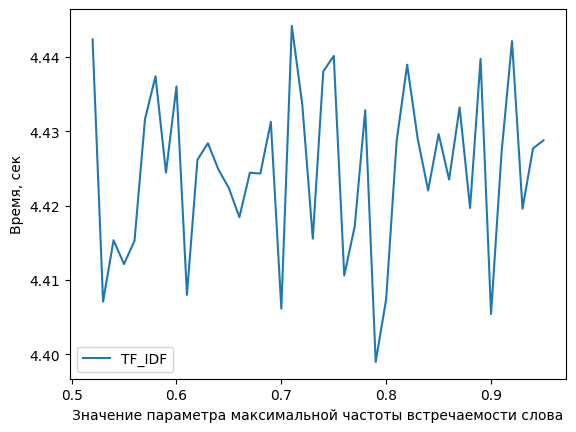
\includegraphics[width=\textwidth]{inc/timesMaxDfTfIdf.png}
	\caption{ График зависимости времени исполнения TF-IDF от значения параметра максимальной частоты встречаемости слова.}
	\label{img:time1}
\end{figure}

\subsection{Зависимость времени исполнения TF-IDF от значения параметра минимальной встречаемости слова}

На рисунке \ref{img:time2} представлен график зависимости времени исполнения TF-IDF от значения параметра минимальной встречаемости слова.

\begin{figure}[H]
	\centering
	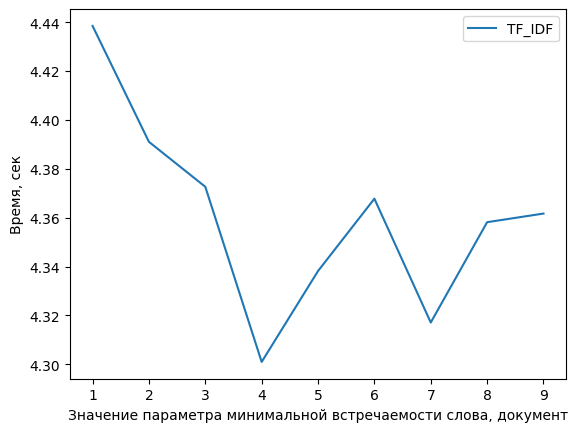
\includegraphics[width=\textwidth]{inc/timesMinDfTfIdf.png}
	\caption{ График зависимости времени исполнения TF-IDF от значения параметра минимальной встречаемости слова.}
	\label{img:time2}
\end{figure}

\subsection{Зависимость времени исполнения LDA от значения параметра количества тем}

На рисунке \ref{img:time3} представлен график зависимости времени исполнения LDA от значения параметра количества тем с разделением по методу обучения.

\begin{figure}[H]
	\centering
	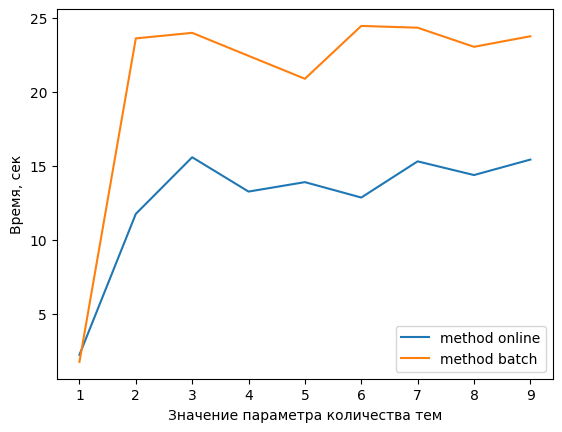
\includegraphics[width=\textwidth]{inc/timesTopicsLda.png}
	\caption{ График зависимости времени исполнения LDA от значения параметра количества тем.}
	\label{img:time3}
\end{figure}

\subsection{Зависимость времени исполнения LDA от значения параметра количества эпох}

На рисунке \ref{img:time4} представлен график зависимости времени исполнения LDA от значения параметра количества эпох с разделением по методу обучения.

\begin{figure}[H]
	\centering
	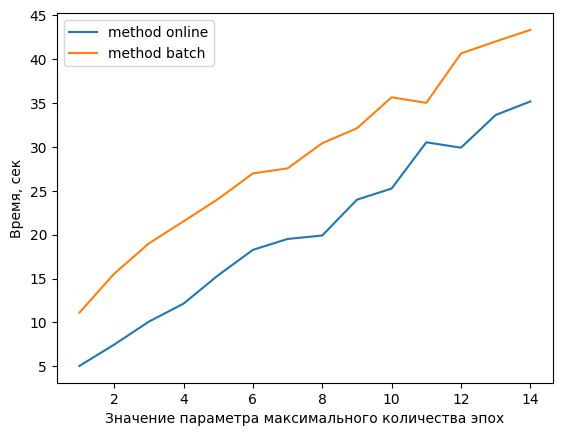
\includegraphics[width=\textwidth]{inc/timesEpochesLda.png}
	\caption{ График зависимости времени исполнения LDA от значения параметра количества эпох.}
	\label{img:time4}
\end{figure}

\subsection*{Заключение}

В результате проведенных исследований легко заметить, что даже при факте включения во время исполнения предобработки данных, TF-IDF в среднем на данном датасете показал себя в $\approx 5$ раз быстрее LDA.

Также можно увидеть, что в LDA лучше всего себя показал метод обучения ``online''. При этом, что ожидаемо, при увеличении количества тем или эпох время исполнения алгоритма увеличивается.